\documentclass[11pt]{article}
\usepackage[margin=1.1in]{geometry}
\usepackage{amsmath,amssymb}
\usepackage{booktabs}
\usepackage[round]{natbib}
\usepackage{graphicx}
\usepackage[hidelinks]{hyperref}
\usepackage{microtype}

\title{Do Hidden Markov Regimes Add Out-of-Sample Value?\\
\large Point forecasts, densities, and tail risk across equities and
commodities}
\author{Anupam Prabhugouda Patil\thanks{apati077@ucr.edu. Code, data and every
number in this paper are reproducible from
\url{https://github.com/jarvisss007/regime-monte-carlo}
(\texttt{run\_full\_study.py}); the test suite re-verifies the
implementations---including recovery of known hidden states and known GARCH
dynamics on synthetic data---in CI on every commit.}}
\date{July 2026}

\begin{document}
\maketitle

\begin{abstract}
\noindent Hidden Markov models (HMMs) occupy a storied place in quantitative
finance: the Baum--Welch algorithm was co-invented by Leonard Baum, Jim
Simons' first partner at Renaissance Technologies. We ask a deliberately
sceptical question: on daily data, does a Gaussian HMM add
\emph{out-of-sample} value over standard volatility filters? We evaluate a
from-scratch three-state HMM against rule-based regimes, RiskMetrics EWMA,
rolling variance, and GARCH(1,1) on three assets (S\&P~500 and NASDAQ,
1999--2018; WTI crude, 1986--2019), in an expanding-window walk-forward with
quarterly refits and 3{,}770--7{,}060 out-of-sample days per asset, scoring
\emph{three distinct objects}: variance point forecasts (QLIKE), the full
predictive density (log score), and 1\% Value-at-Risk (Kupiec and
Christoffersen backtests). The answer depends on what is scored. For point
variance, smooth conditional-variance recursions win: GARCH(1,1) is best on
all three assets and EWMA second, both significantly ahead of the HMM on
equities (Diebold--Mariano $t\approx2$). For densities, the HMM closes the
gap---statistically indistinguishable from EWMA on equities---and wins
outright on the fat-tailed commodity ($t=-3.1$). For tail risk the ranking
inverts decisively: every Gaussian forecaster materially over-breaches a
1\% VaR (up to 2.6\% hit rates), while the HMM mixture has the lowest breach
rate on all three assets and is the \emph{only} model anywhere with
statistically correct coverage (WTI, Kupiec $p=0.38$). Descriptively, the
HMM discovers the leverage effect unsupervised---its calm state drifts up,
its turbulent state drifts down. Volatility-targeting overlays raise Sharpe
ratios on the equity indices but no improvement survives a stationary
block-bootstrap test. The conclusion is a division of labour: hidden-state
mixtures are \emph{risk} models---tails, densities, description---while
one-parameter recursions remain better \emph{point} forecasters.
Sophistication is not edge; it is insurance.
\end{abstract}

\section{Introduction}
The romance of regime-switching models in finance begins with a
biographical fact: before founding Renaissance Technologies, Jim Simons
partnered with Leonard Baum, co-inventor of the algorithm
\citep{baum1970} that made hidden Markov models estimable. The intellectual
bet---that markets, like speech, are driven by unobservable states that can
be inferred from noisy observations---has attracted researchers ever since
\citep{hamilton1989, ryden1998, ang2002, guidolin2007, nystrup2018}.

This paper asks the question an allocator (or a sceptical PhD committee)
would ask: \emph{does the machinery pay its way out of sample?} And it
insists on a distinction the literature often blurs: ``forecasting
volatility'' is not one task but several. A model may forecast the
\emph{level} of tomorrow's variance poorly while describing the
\emph{shape} of tomorrow's return distribution well---and for a risk
manager the shape, especially the left tail, is the object that matters.
We therefore score every model on three progressively richer objects:
variance point forecasts under QLIKE loss \citep{patton2011}, the full
one-day-ahead predictive density under the logarithmic score, and 1\%
Value-at-Risk under formal coverage and independence backtests
\citep{kupiec1995, christoffersen1998}.

Our contribution is not a new model but an honest accounting, in the spirit
of \citet{hansen2005}, who asked whether anything beats a GARCH(1,1). On
the point-forecast leg our answer agrees with theirs; on the tail-risk leg
it reverses. That reversal---sophistication losing the forecasting race
while winning the risk race---is the paper's central finding.

\section{Models}
\subsection{Gaussian hidden Markov model}
Daily returns $r_t$ are modelled as draws from one of $K$ Gaussian
emission distributions $\mathcal{N}(\mu_k,\sigma_k^2)$, selected by a latent
first-order Markov chain $s_t$ with transition matrix $A$. Parameters
$(\pi, A, \mu, \sigma)$ are estimated by Baum--Welch
(expectation--maximisation over scaled forward--backward recursions),
implemented from scratch; the most likely state path is decoded by Viterbi.
Initialisation is deterministic (quantile splits of $|r_t|$), and states are
relabelled by ascending $\sigma_k$. Correctness is verified on synthetic
data with \emph{known} hidden states before any market data is touched: the
implementation recovers the true path with $>85\%$ Viterbi accuracy and the
true $\sigma_k$ within 15\%. Our baseline uses $K=3$; Section~\ref{sec:k}
varies $K$.

For out-of-sample use we maintain the filtered distribution
$p_t = P(s_t \mid r_{1:t})$ recursively. With predictive mixture weights
$q = p_t A$, the one-day-ahead density is the mixture
$\sum_k q_k\,\mathcal{N}(\mu_k,\sigma_k^2)$; its variance is
\begin{equation}
\widehat{\text{Var}}_t(r_{t+1}) = \sum_k q_k(\sigma_k^2 + \mu_k^2)
- \Big(\sum_k q_k \mu_k\Big)^2,
\end{equation}
and its $\alpha$-quantile (for VaR) is obtained by bisection on the mixture
CDF. The HMM is thus the only model in the comparison whose predictive
density is non-Gaussian.

\subsection{Comparators}
\textbf{Rule-based regimes:} days classified calm/normal/turbulent by
terciles of trailing 21-day realised volatility (tercile edges from training
data only); the forecast is the training-sample variance of the current
regime's return pool---the observable-state analogue of the HMM.
\textbf{EWMA:} $\hat v_{t+1} = 0.94\,\hat v_t + 0.06\,r_t^2$
\citep{riskmetrics1996}.
\textbf{Rolling:} 21-day trailing variance.
\textbf{GARCH(1,1):} $\hat v_{t+1} = \omega + \alpha r_t^2 + \beta \hat
v_t$ with zero mean, estimated by maximum likelihood at each refit
\citep{bollerslev1986}; between refits the recursion runs with fixed
parameters. (Our estimator recovers known $(\alpha,\beta)$ on simulated
GARCH data within tight tolerances; this is part of the test suite.)
The four comparators produce Gaussian predictive densities
$\mathcal{N}(0,\hat v_{t+1})$; note that for Gaussian densities the log
score is an affine transform of QLIKE, so their density ranking must match
their QLIKE ranking---only the HMM can genuinely differ across the two.

\section{Data and protocol}
Assets are daily closes bundled with the open-source \texttt{arch} package
(no vendor access): S\&P~500 and NASDAQ composite (January 1999--December
2018) and WTI crude spot (1986--2019). The first 1{,}260 trading days form
the initial estimation window; all models are re-estimated every 63 days on
an expanding window; filters and recursions update daily. Every forecast of
day $t{+}1$ uses only information through day $t$. This yields 3{,}770
out-of-sample days for each equity index and 7{,}060 for WTI. Point
forecasts are scored by QLIKE, $L_t = \log\hat v_t + r_t^2/\hat v_t$,
robust to noisy volatility proxies \citep{patton2011}; densities by the log
score; forecast differences tested by Diebold--Mariano statistics with a
Bartlett/HAC variance at five lags \citep{diebold1995}. VaR calibration is
tested by Kupiec's proportion-of-failures likelihood ratio
\citep{kupiec1995} and Christoffersen's independence test
\citep{christoffersen1998}.

\section{Results}
\subsection{What the HMM discovers}
Fitted to the full S\&P sample, the three states are not mere volatility
buckets (Table~\ref{tab:states}): mean returns fall monotonically as
volatility rises, from a calm state combining a $+9.2$\,bp daily drift with
8.7\% annualised volatility to a turbulent state combining $-11.5$\,bp with
42.2\%. The model was never shown a volatility feature or a sign
asymmetry---it inferred the leverage effect from raw returns, consistent
with \citet{ryden1998}. States are highly persistent (expected durations
32--49 trading days) and the chain never transits directly between calm and
turbulent: panic arrives, and recedes, through the intermediate state.

\begin{table}[t]
\centering
\caption{Three-state Gaussian HMM, S\&P 500 daily returns, 1999--2018.}
\label{tab:states}
\begin{tabular}{lrrrr}
\toprule
state & $\mu_k$ (bp/day) & $\sigma_k$ (ann.) & self-persistence & E[duration] \\
\midrule
calm      & $+9.2$  & 8.7\%  & 0.979 & 48.5 days \\
normal    & $-1.8$  & 18.5\% & 0.973 & 37.4 days \\
turbulent & $-11.5$ & 42.2\% & 0.969 & 31.8 days \\
\bottomrule
\end{tabular}
\end{table}

\begin{figure}[t]
\centering
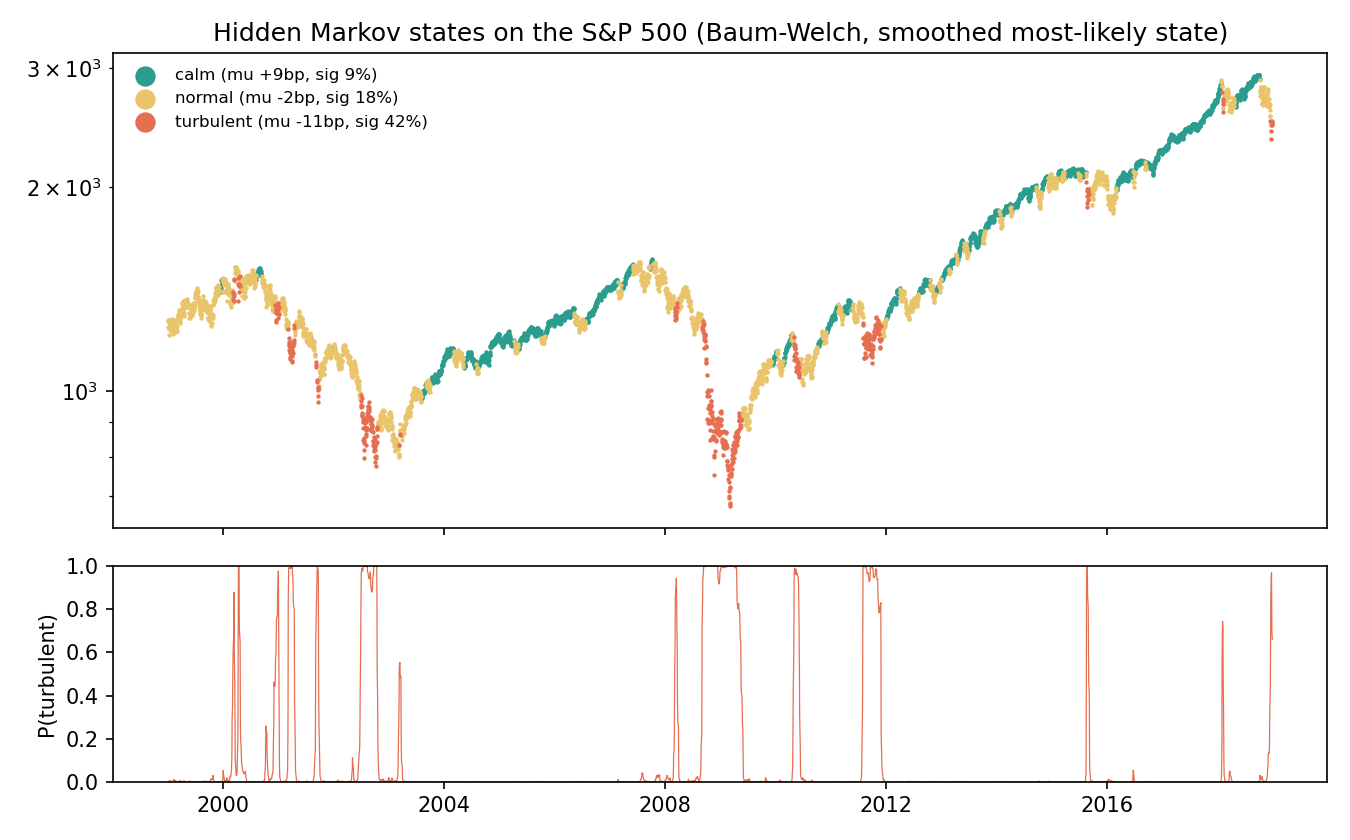
\includegraphics[width=\textwidth]{../figures/fig5_hmm_states.png}
\caption{Top: S\&P 500 (log scale) coloured by decoded hidden state.
Bottom: smoothed probability of the turbulent state.}
\label{fig:states}
\end{figure}

\subsection{Point forecasts: smooth recursions win}
Table~\ref{tab:qlike} reports QLIKE across all assets. The ordering is
strikingly stable: GARCH(1,1) first on all three assets---significantly
ahead of even the EWMA on both equity indices ($t=-2.1,\,-2.2$)---EWMA
second, the HMM third, and the piecewise-constant forecasters (rolling,
rule-based) last, decisively so ($t$ up to 9.3). The HMM's deficit to the
EWMA is significant on the S\&P ($t=2.0$), marginal on NASDAQ ($t=1.8$),
and insignificant on WTI ($t=0.9$).

The mechanism is structural. Regime forecasts are piecewise-constant:
within a regime the forecast barely moves; across the boundary it jumps
between a small number of levels. Conditional variance itself evolves
continuously, and the geometric weighting of GARCH/EWMA tracks that
evolution day by day, while a three-state mixture must express all
variation through shifts in $q$.

\begin{table}[t]
\centering
\caption{Variance point forecasts: QLIKE (lower is better) and
Diebold--Mariano $t$ against the EWMA benchmark (positive $=$ EWMA more
accurate). Out-of-sample days: 3{,}770 (S\&P, NASDAQ), 7{,}060 (WTI).}
\label{tab:qlike}
\begin{tabular}{lrrrrrr}
\toprule
& \multicolumn{2}{c}{S\&P 500} & \multicolumn{2}{c}{NASDAQ}
& \multicolumn{2}{c}{WTI} \\
forecaster & QLIKE & $t$ & QLIKE & $t$ & QLIKE & $t$ \\
\midrule
GARCH(1,1)        & $\mathbf{-8.462}$ & $-2.1$ & $\mathbf{-8.099}$ & $-2.2$ & $\mathbf{-6.723}$ & $-1.4$ \\
EWMA(0.94)        & $-8.435$ & ---    & $-8.082$ & ---    & $-6.714$ & --- \\
HMM mixture       & $-8.357$ & $2.0$  & $-8.056$ & $1.8$  & $-6.705$ & $0.9$ \\
21-day rolling    & $-8.378$ & $4.1$  & $-8.031$ & $4.1$  & $-6.675$ & $5.7$ \\
rule-based regimes& $-8.350$ & $2.7$  & $-8.031$ & $3.6$  & $-6.600$ & $9.3$ \\
\bottomrule
\end{tabular}
\end{table}

\subsection{Densities: the mixture closes the gap}
Scoring the full predictive density (Table~\ref{tab:logscore}) changes the
HMM's standing. Against the EWMA it is statistically indistinguishable on
both equity indices ($t=0.9,\,0.3$)---the fat-tailed mixture recovers on
density exactly what its variance point forecast loses---and on WTI, the
fattest-tailed asset in the panel, it is significantly \emph{better}
($t=-3.1$), overtaking GARCH for first place. For the Gaussian comparators
the density ranking is mechanically identical to the QLIKE ranking (the log
score of a Gaussian is affine in QLIKE); the HMM is the only model able to
improve its rank between the two tables, and it does.

\begin{table}[t]
\centering
\caption{Predictive density: mean log score (higher is better); DM $t$
against EWMA on the negative log-score loss (negative $=$ model beats
EWMA).}
\label{tab:logscore}
\begin{tabular}{lrrrrrr}
\toprule
& \multicolumn{2}{c}{S\&P 500} & \multicolumn{2}{c}{NASDAQ}
& \multicolumn{2}{c}{WTI} \\
forecaster & score & $t$ & score & $t$ & score & $t$ \\
\midrule
GARCH(1,1)        & $\mathbf{3.312}$ & $-2.1$ & $\mathbf{3.131}$ & $-2.2$ & $2.443$ & $-1.4$ \\
EWMA(0.94)        & $3.298$ & ---    & $3.122$ & ---    & $2.438$ & --- \\
HMM mixture       & $3.280$ & $0.9$  & $3.120$ & $0.3$  & $\mathbf{2.460}$ & $\mathbf{-3.1}$ \\
21-day rolling    & $3.270$ & $4.1$  & $3.096$ & $4.1$  & $2.419$ & $5.7$ \\
rule-based regimes& $3.256$ & $2.7$  & $3.096$ & $3.6$  & $2.381$ & $9.3$ \\
\bottomrule
\end{tabular}
\end{table}

\subsection{Tail risk: the ranking inverts}
Table~\ref{tab:var} contains the paper's sharpest result. At a 1\% VaR
target, every Gaussian forecaster over-breaches on every asset---hit rates
of 1.5\%--2.6\%, i.e.\ 50\%--160\% more tail events than promised, with
Kupiec rejections at $p<10^{-4}$ throughout. The HMM mixture has the lowest
breach rate on all three assets (1.56\%, 1.62\%, 1.10\%) and on WTI it is
the \emph{only} model in the entire study whose coverage cannot be rejected
(Kupiec $p=0.38$; Christoffersen independence $p=0.19$). The economic
reading: a Gaussian tail hung on even the best point forecast of variance
is the wrong shape, and the error is first-order for risk management. The
mixture's overweighting of the turbulent component buys exactly the tail
mass that Gaussian models lack. The HMM is not perfect---on the S\&P its
breaches cluster (Christoffersen $p=0.002$), betraying regime
transitions detected with a lag---but it dominates the alternatives on
calibration everywhere.

\begin{table}[t]
\centering
\caption{1\% one-day VaR backtests. Hit rate should equal 1\%. K-$p$:
Kupiec coverage $p$-value (higher is better; $\geq0.05$ means calibration
cannot be rejected). C-$p$: Christoffersen independence $p$-value.}
\label{tab:var}
\begin{tabular}{lrrrrrrrrr}
\toprule
& \multicolumn{3}{c}{S\&P 500} & \multicolumn{3}{c}{NASDAQ}
& \multicolumn{3}{c}{WTI} \\
forecaster & hit\% & K-$p$ & C-$p$ & hit\% & K-$p$ & C-$p$ & hit\% & K-$p$ & C-$p$ \\
\midrule
HMM mixture  & $\mathbf{1.56}$ & .001 & .002 & $\mathbf{1.62}$ & .000 & .361
             & $\mathbf{1.10}$ & $\mathbf{.384}$ & .187 \\
GARCH(1,1)   & 1.75 & .000 & .143 & 1.78 & .000 & .155 & 1.47 & .000 & .714 \\
EWMA(0.94)   & 2.23 & .000 & .437 & 1.96 & .000 & .250 & 1.74 & .000 & .248 \\
rule-based   & 2.44 & .000 & .032 & 1.86 & .000 & .192 & 2.12 & .000 & .006 \\
21-day rolling & 2.60 & .000 & .017 & 2.47 & .000 & .648 & 2.05 & .000 & .565 \\
\bottomrule
\end{tabular}
\end{table}

\subsection{State-count sensitivity}\label{sec:k}
Re-running the S\&P walk-forward with $K\in\{2,3,4\}$ improves both scores
monotonically in $K$: QLIKE moves from $-8.317$ ($K{=}2$) to $-8.357$
($K{=}3$) to $-8.429$ ($K{=}4$), the last within a whisker of the EWMA's
$-8.435$; the log score rises from 3.253 to 3.280 to 3.316, at $K{=}4$
exceeding both EWMA (3.298) and GARCH (3.312). A finer state grid
approximates a continuous volatility process better, converging toward the
smooth-recursion benchmarks---which clarifies that the three-state model's
point-forecast deficit is a discretisation cost, not a flaw of the
hidden-state idea.

\subsection{Does it cash out? Volatility targeting, honestly tested}
Finally we ask whether any of this matters for a simple investor via a
10\%-annualised-vol-target overlay, $w_t = \min(1,
\sigma_{\text{tgt}}/\hat\sigma_t)$, net of 2\,bps per side on turnover
\citep{moreira2017}. On the equity indices every forecaster's overlay
raises the Sharpe ratio (S\&P: 0.38 buy-and-hold $\to$ 0.42--0.51; NASDAQ:
0.48 $\to$ 0.55--0.64) and roughly halves maximum drawdown (S\&P $-57\%\to
-25\%$; NASDAQ $-56\%\to-22\%$). But a stationary block-bootstrap test of
the Sharpe difference \citep{politis1994} rejects nothing: the smallest
$p$-value in the panel is 0.10, and on WTI the overlays fail to beat
buy-and-hold at all. Forecast-accuracy differences between overlay drivers
are second-order relative to the sampling variation of Sharpe ratios over
two decades. We report this as an honest null: volatility targeting
\emph{looks} valuable, its drawdown reduction is large and mechanical, but
its Sharpe improvement on this sample does not clear conventional
significance---and it certainly provides no wedge for sophisticated
volatility models over simple ones.

\section{Discussion}
The three scoring rules assemble into one coherent picture. Conditional
variance is nearly a continuous-path process; models whose forecasts move
smoothly with every observation (GARCH, EWMA) track its level best, and no
amount of hidden-state elegance changes that---consistent with
\citet{hansen2005}, and now shown to extend to HMMs across asset classes.
But the \emph{conditional distribution} of returns is not Gaussian, and
here the mixture structure earns its keep: matching Gaussian benchmarks on
equity densities, beating them on commodity densities, and delivering the
only correctly calibrated 1\% VaR in the study. The hidden-state model is
best understood not as a forecaster but as a risk model---a machine for
getting the tail right---and, descriptively, as an unsupervised discoverer
of economically meaningful structure (the leverage effect, regime
persistence, the no-direct-jump topology of market stress). The
Renaissance lesson survives in amended form: the mathematics of Baum
genuinely sees structure that simple filters do not; converting that
structure into point-forecast dominance---let alone into edge---is another
matter entirely.

\section{Limitations}
(i)~Gaussian emissions; Student-$t$ emissions would likely sharpen both
density and VaR results and might close the remaining coverage gap on
equities. (ii)~$K{\leq}4$; Section~\ref{sec:k} suggests larger $K$
converges toward smooth filters, a trade-off worth mapping fully.
(iii)~Quarterly refits are a compute compromise. (iv)~Three assets, daily
frequency, one VaR level; intraday data and multi-asset joint modelling are
the natural extensions. (v)~The overlay analysis uses one target and one
cost assumption; its null should be read as absence of evidence at this
sample size, not proof of absence.

\section{Conclusion}
Evaluated honestly and out of sample, a Gaussian hidden Markov model on
daily returns is a mediocre point forecaster, a competitive density
forecaster, the best tail-risk model in its comparison set, and a genuinely
insightful descriptive device. The one-parameter EWMA and GARCH(1,1) remain
the right tools for predicting tomorrow's variance level; the hidden-state
mixture is the right tool when the question is how bad tomorrow can get.
What one concludes about ``sophistication'' in quantitative finance
depends entirely on the scoring rule---which is, perhaps, the most
practical lesson this study has to offer.

\section*{Reproducibility}
\texttt{python run\_full\_study.py} reproduces Tables 2--5 and the overlay
results; \texttt{python run\_hmm\_study.py} reproduces Table~1;
\texttt{python plots\_hmm.py} reproduces Figure~1; \texttt{pytest} (17
tests) re-verifies the HMM, GARCH, and backtest implementations against
synthetic data with known properties, in CI on every commit. Data ship
with the \texttt{arch} package; no vendor access is required.

\begin{thebibliography}{15}
\bibitem[Ang \& Bekaert(2002)]{ang2002}
Ang, A., \& Bekaert, G. (2002). International asset allocation with
regime shifts. \emph{Review of Financial Studies}, 15(4), 1137--1187.

\bibitem[Baum et al.(1970)]{baum1970}
Baum, L.~E., Petrie, T., Soules, G., \& Weiss, N. (1970). A maximization
technique occurring in the statistical analysis of probabilistic functions
of Markov chains. \emph{Annals of Mathematical Statistics}, 41(1), 164--171.

\bibitem[Bollerslev(1986)]{bollerslev1986}
Bollerslev, T. (1986). Generalized autoregressive conditional
heteroskedasticity. \emph{Journal of Econometrics}, 31(3), 307--327.

\bibitem[Christoffersen(1998)]{christoffersen1998}
Christoffersen, P.~F. (1998). Evaluating interval forecasts.
\emph{International Economic Review}, 39(4), 841--862.

\bibitem[Diebold \& Mariano(1995)]{diebold1995}
Diebold, F.~X., \& Mariano, R.~S. (1995). Comparing predictive accuracy.
\emph{Journal of Business \& Economic Statistics}, 13(3), 253--263.

\bibitem[Guidolin \& Timmermann(2007)]{guidolin2007}
Guidolin, M., \& Timmermann, A. (2007). Asset allocation under multivariate
regime switching. \emph{Journal of Economic Dynamics and Control}, 31(11),
3503--3544.

\bibitem[Hamilton(1989)]{hamilton1989}
Hamilton, J.~D. (1989). A new approach to the economic analysis of
nonstationary time series and the business cycle. \emph{Econometrica},
57(2), 357--384.

\bibitem[Hansen \& Lunde(2005)]{hansen2005}
Hansen, P.~R., \& Lunde, A. (2005). A forecast comparison of volatility
models: does anything beat a GARCH(1,1)? \emph{Journal of Applied
Econometrics}, 20(7), 873--889.

\bibitem[Kupiec(1995)]{kupiec1995}
Kupiec, P.~H. (1995). Techniques for verifying the accuracy of risk
measurement models. \emph{Journal of Derivatives}, 3(2), 73--84.

\bibitem[Moreira \& Muir(2017)]{moreira2017}
Moreira, A., \& Muir, T. (2017). Volatility-managed portfolios.
\emph{Journal of Finance}, 72(4), 1611--1644.

\bibitem[Nystrup et al.(2018)]{nystrup2018}
Nystrup, P., Madsen, H., \& Lindstr\"om, E. (2018). Dynamic portfolio
optimization across hidden market regimes. \emph{Quantitative Finance},
18(1), 83--95.

\bibitem[Patton(2011)]{patton2011}
Patton, A.~J. (2011). Volatility forecast comparison using imperfect
volatility proxies. \emph{Journal of Econometrics}, 160(1), 246--256.

\bibitem[Politis \& Romano(1994)]{politis1994}
Politis, D.~N., \& Romano, J.~P. (1994). The stationary bootstrap.
\emph{Journal of the American Statistical Association}, 89(428),
1303--1313.

\bibitem[RiskMetrics(1996)]{riskmetrics1996}
J.P.~Morgan/Reuters (1996). \emph{RiskMetrics---Technical Document},
4th~ed. New York.

\bibitem[Ryd\'en et al.(1998)]{ryden1998}
Ryd\'en, T., Ter\"asvirta, T., \& \AA sbrink, S. (1998). Stylized facts of
daily return series and the hidden Markov model. \emph{Journal of Applied
Econometrics}, 13(3), 217--244.
\end{thebibliography}

\end{document}
